\subsubsection{UC35 - Visualizzazione contenuto prompt generato}\label{UC35}

\begin{figure}[H]
  \centering
  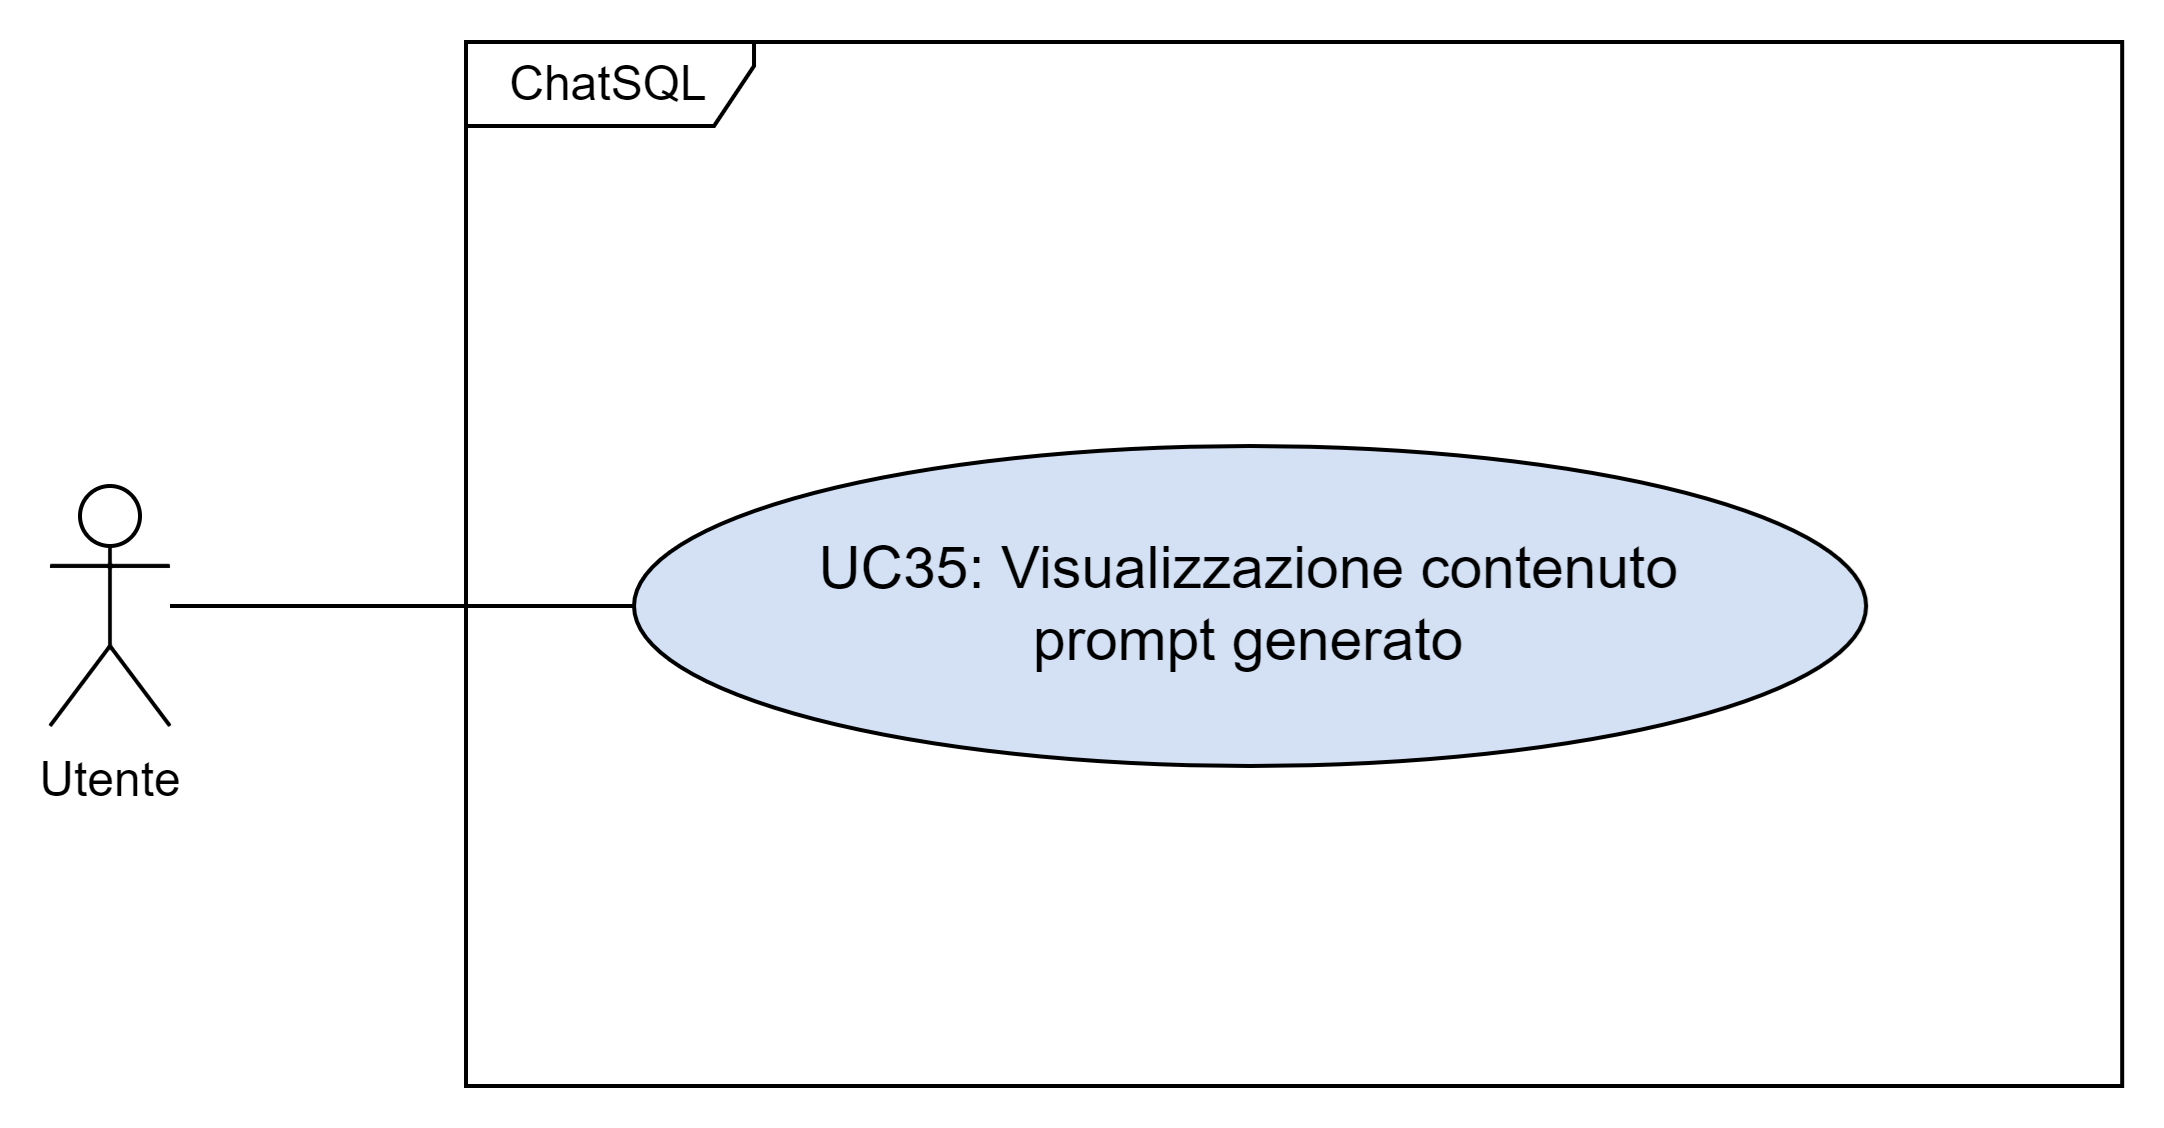
\includegraphics[width=0.90\textwidth]{assets/uc35.png}
  \caption{UC35}
\end{figure}

\paragraph*{Descrizione}
L'Utente visualizza il contenuto del \glossario{prompt} generato.

\paragraph*{Attori principali}
Utente

\paragraph*{Precondizioni}
\begin{itemize}
  \item Il sistema è attivo e funzionante;
  \item È stato generato almeno un \glossario{prompt}.
\end{itemize}

\paragraph*{Postcondizioni}
\begin{itemize}
  \item Viene visualizzato correttamente il contenuto del \glossario{prompt}.
\end{itemize}

\paragraph*{Trigger}
L'Utente vuole visualizzare il contenuto di un \glossario{prompt}.

\paragraph*{Scenario principale}
\begin{enumerate}
  \item L'Utente visualizza il contenuto del \glossario{prompt};
  \item Il sistema mostra le seguenti informazioni:
  \begin{itemize}
    \item Legenda dei simboli utilizzati nel \glossario{prompt};
    \item Lista delle tabelle pertinenti:
    \begin{itemize}
      \item Schema della tabella;
      \item Chiave primaria;
      \item Descrizione della tabella;
      \item Descrizione delle colonne della tabella;
      \item Chiavi esterne;
    \end{itemize}
    \item DBMS di riferimento;
    \item Lingua di riferimento;
    \item Richiesta il linguaggio naturale.
  \end{itemize}
\end{enumerate}
